\documentclass{book}
\usepackage{tikz-cd}
\usepackage{tikz}
\usetikzlibrary{arrows}

\newcommand{\Dcal}{\mathcal{D}}

\begin{document}

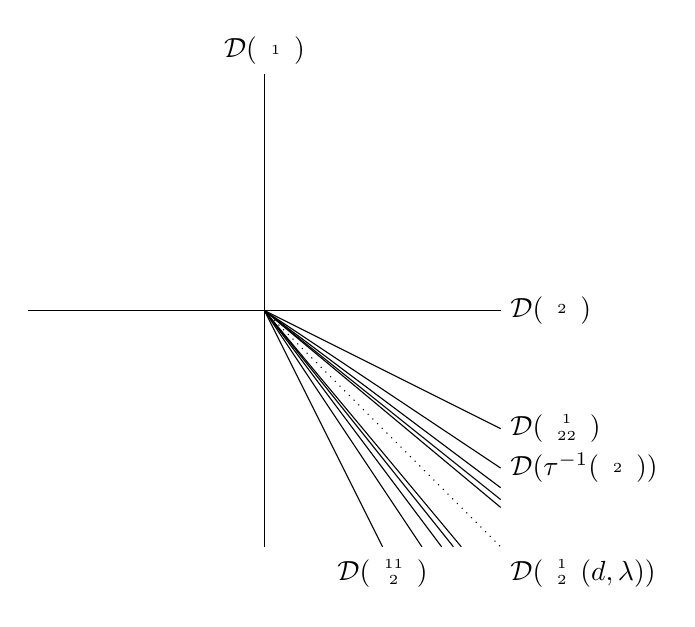
\begin{tikzpicture}
  \draw[-] (-3, 0) -- (3, 0) node[right] {$\Dcal({\tiny \begin{array}{c} 2 \end{array}})$};
  \draw[-] (0, -3) -- (0, 3) node[above] {$\Dcal({\tiny \begin{array}{c} 1 \end{array}})$};
  \draw[-] (0,0) -- (3,-1.5) node[right] {$\Dcal(\tiny{\begin{array}{cc} 1 \\22 \end{array}}\normalsize)$};
  \draw[-] (0,0) -- (3,-2) node[right] {$\Dcal(\tau^{-1}({\tiny \begin{array}{c}  2 \end{array}}))$};
  \draw[-] (0,0) -- (3,-9/4);
  \draw[-] (0,0) -- (3,-12/5);
  \draw[-] (0,0) -- (3,-2.5);
  \draw[dotted] (0,0) -- (3,-3) node[below right] {$\Dcal(\tiny{\begin{array}{cc} 1 \\2 \end{array}}\normalsize(d,\lambda))$};
  \draw[-] (0,0) -- (2.5,-3);
  \draw[-] (0,0) -- (12/5,-3);
  \draw[-] (0,0) -- (9/4,-3);
  \draw[-] (0,0) -- (2,-3);
  \draw[-] (0,0) -- (1.5,-3) node[below] {$\Dcal(\tiny{\begin{array}{cc} 11 \\2 \end{array}}\normalsize)$};
\end{tikzpicture}

\end{document}